\documentclass[11pt,a4paper]{article}
\usepackage{fontspec}
\setmainfont{Noto Serif CJK SC}
\setsansfont{Noto Sans CJK SC}
\setmonofont{DejaVu Sans Mono}
\XeTeXlinebreaklocale "zh"
\XeTeXlinebreakskip=0pt plus 1pt
\usepackage[margin=22mm]{geometry}
\usepackage{amsmath,amssymb,booktabs,graphicx,xcolor,hyperref,fancyhdr}
\hypersetup{colorlinks=true,urlcolor=blue,linkcolor=blue,pdftitle={LTN扩散与掺混：周期接触oracle判别},pdfauthor={diffuse-mixing research}}
\setlength{\parindent}{0pt}\setlength{\parskip}{6pt}
\pagestyle{fancy}\fancyhf{}\fancyhead[L]{\small diffuse-mixing / LTN}\fancyhead[R]{\small 2026-11-04}\fancyfoot[C]{\thepage}
\setlength{\headheight}{16pt}
\begin{document}
\begin{center}{\LARGE\bfseries LTN扩散与掺混}\par\vspace{3mm}{\Large 同一普通FV周期接触oracle判别}\par\vspace{3mm}2026年11月4日（Asia/Shanghai）\end{center}
\section*{1. 本轮结论与项目位置}
\textbf{N32同一后端静止周期接触oracle判别通过。Stage 3仍未完整通过，fluid ORC保持关闭，未计算曲率。}

本轮承接已封存的T3仿射剪切三档空间对照，执行其唯一下一项。新环境能够读取旧成果；上一轮约22 MB交付包与6374条累计科学哈希逐项核对保持。没有重新应用旧修改、重跑旧候选或发布环境/版本。PDF与代码压缩包是本轮用户明确要求的下载交付。

\begin{center}\begin{tabular}{p{35mm}p{111mm}}\toprule
项目 & 当前证据与限制\\\midrule
T1与T2 & 已封存均匀扩散、平移、D=0与精确旋转控制；本轮不重跑。\\
T3仿射压缩/剪切 & 给定算例的方向、本构与三空间档登记覆盖已补齐。不是一般点云收敛定理。\\
本轮T4接触 & 一张N32静态点几何图，实际K16传播与完整独立控制及Cartesian全模态半离散解相容。\\
剩余T4工作 & 本接触必要三档空间控制、最终同后端移动激波、三密度来源闭合。\\
Stage 3 / ORC & incomplete；fluid ORC关闭。当前研究指数作用与原默认隐式Euler交付范围区分。\\\bottomrule
\end{tabular}\end{center}

固定单位周期方形、等半两相$\rho_L=1,\rho_R=4$、原二进制$D=0.02$、$T=1/20$。$N=32$代表$32\times32=1024$个固定物质单元。接触位于$x=1/2$及周期接缝；不是开放边界移动激波。

\textbf{终时相对PDE误差：0.00043411079；相对独立Cartesian传播差：7.1422453e-15。} 两者量级分离，支持该有限算例中的几何/阻力/传播实现衔接。单N32误差不能替代空间收敛或完整T4验收；没有据结果重新设置物理精度阈值。

本轮新增三项软件检查经复核通过，累计记录493项，旧490项未重跑。首次夹具与审计失败及其修正均保留。旧v0.8.0/246仍未恢复，不冒称当前代码是取回的旧版本。
\newpage
\section*{2. 物质平均、几何与透射参考}
\subsection*{2.1 固定质量未知量与普通阻力}
\[
m_i=\int_{K_i}\rho\,dV,\qquad \bar c_i=\frac1{m_i}\int_{K_i}\rho c\,dV,
\qquad m_i=\frac{\rho_i}{N^2},\quad\sum_i m_i=\frac52.
\]
初值由原连续公式积分新推导，不插值旧N128均值，也不从轨迹点值重采样。图构造器仅接收点、ID、给定oracle点密度、$D$和周期边界；不接收真实物质面、$F/C$或参考标量。\textbf{唯一系数图先封存，再解析实际质量、初值与参考。}
\[
g_{ij}=\frac{|f_{ij}|}{\ell_i/(\rho_iD)+\ell_j/(\rho_jD)}.
\]
本方格相内$g=D,4D$，界面$g=(8/5)D$；这些是封存后核对值，不用于代替点几何构造。2048个共享正面中低相992、高相992、界面64。独立审计重建双中垂线、互反面、两半阻力、面积和固定全点探针。没有删跨界正面、裁剪、重归一化或改质量/密度/初场。

\subsection*{2.2 连续谱与真实有限单元平均}
原初场$c_0=1/2+f_0(x)\cos(2\pi y)$，
\[
f_0(x)=\tfrac15\cos[\pi(a_px+\phi_p)],\quad
(a_L,\phi_L)=(16/5,1/5),\quad(a_R,\phi_R)=(4/5,7/5).
\]
质量加权透射算子$A=-\rho^{-1}(\rho D f')'$的完整基为$1$、$\cos(2\pi nx)$、$\sin(2\pi nx)/\rho(x)$；两接触处$[c]=[\rho D\partial_xc]=0$。令$\tau=4\pi^2Dt$，复用原存128模态90位系数$\alpha_n,\beta_n$：
\[
c=\tfrac12+e^{-\tau}\cos(2\pi y)
\left[\alpha_0+\sum_{n=1}^{128}e^{-\tau n^2}
\left(\alpha_n\cos(2\pi nx)+\beta_n\frac{\sin(2\pi nx)}{\rho}\right)\right].
\]
参考评价逐物质格积分，保留$\operatorname{sinc}$因子与法向常数模态的横向衰减。$t=0$直接积分连续初场，不以有限谱截断替换。初值序列化质量范数桥为4.1146987e-17，原样保留。

Decimal100/120位评价与独立mpmath80/100位核对。原评价指标保持为\[64\epsilon\sqrt M\max(1,\max|c_0|).\]128模态尾项的解析指数下界按$t=0.025$与$0.05$分别计算；不把终时尾界用于更早时刻。算术/舍入控制不冒充区间认证总误差界。
\newpage
\section*{3. 数值结果与误差分离}
误差按原初质量波动归一化，H保持原定义：\[\frac{\|\bar c^{FV}-\bar c^{PDE}\|_m}{\sigma_0},\quad \sigma_0=0.1975185511597745,\quad H=1-\frac{\mathrm{Var}_m(c)}{\mathrm{Var}_m(c_0)}.\]
\begin{center}\small\begin{tabular}{rrrr}\toprule
$t$ & FV/PDE误差 & FV/Cartesian差 & 固定作用指标\\\midrule
0 & 0 & 3.15479e-15 & 2.13593e-12 \\
0.025 & 0.000329137 & 4.85846e-15 & 7.88852e-11 \\
0.05 & 0.000434111 & 7.14225e-15 & 1.55633e-10 \\
\bottomrule\end{tabular}\end{center}
\begin{center}\small\begin{tabular}{rrrr}\toprule
$t$ & 实际$H$ & PDE参考$H$ & 原始质量漂移\\\midrule
0 & 0.000000000000 & 0.000000000000 & 0 \\
0.025 & 0.053491095542 & 0.053676537790 & -1.3048e-16 \\
0.05 & 0.103559525616 & 0.103898997327 & -3.3025e-16 \\
\bottomrule\end{tabular}\end{center}
\begin{center}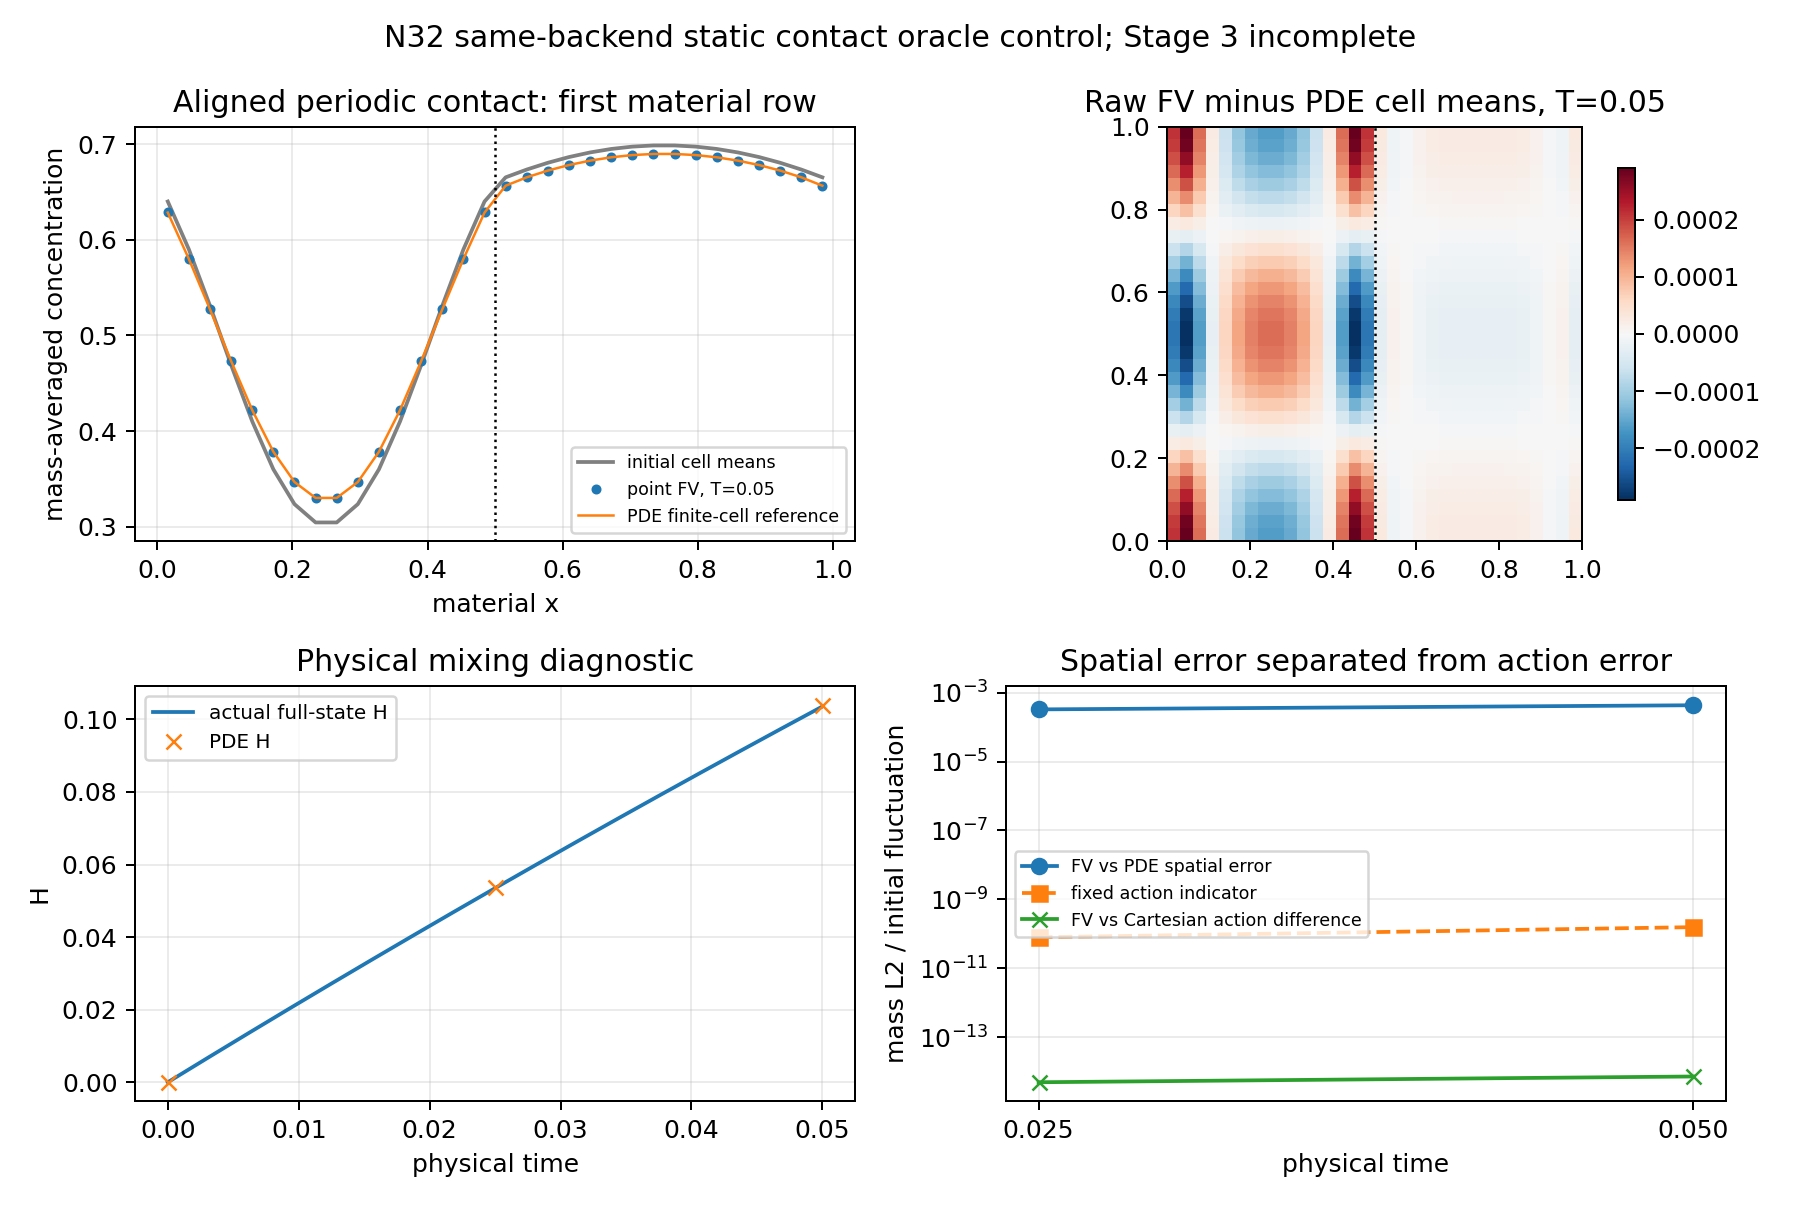
\includegraphics[width=.94\textwidth]{contact-oracle.png}\end{center}
主路径使用同一稀疏指数作用与完整正统一化，原权重不归一化。静态$L$没有中点冻结误差，因此不制造4/8/16时间下降要求。独立Cartesian控制保留全部1024离散模态及原始c0；法向32阶原始最小特征值不置零。另从精确两半阻力重建法向环，用Padé指数核对全部17个端点。

PDE误差分解保留独立半离散空间项、原作用数值项、参考评价/尾项及初态桥，逐项正加；$H$使用原二次扰动指标。没有有符号抵消、拟合参数或浓度外推。
\newpage
\section*{4. 审计、保全与重放}
\textbf{主计算首次完成：2.919秒／65.84 MiB。} 在900秒／1024 MiB资源封顶内。原始库存、极值、质量方差、正性与共享面耗散按原代数尺度检查；最大原始质量漂移3.3024798e-16，未调平。

\textbf{软件检查：} 首次3项中几何夹具N4的$L^1$半径恰为$1/4$，不满足旧审计严格$R<1/4$条件；只把该夹具改为N8及对应探针/面数。原失败源码、JSON与日志保留，未改审计门槛或N32科学算例。第二次3项均通过。另含独立Gauss有限均值积分、分时尾项、扰坏完整序列与Cartesian状态后的拒绝检查。

\textbf{报告类型恢复：} 首次完整审计在JSON字值核对处失败：原Cartesian总指标为NumPy float64，JSON读回Python float后，Python3.12补偿sum与原顺序NumPy sum产生末位差。原科学代码、结果和48个恢复前文件保持。追加入口仅恢复原标量类型，IEEE值位不变，同一冻结evaluate精确复现原结果。没有增大指标或改阈值，不重算科学路径。第二次完整审计通过：26.508秒／68.51 MiB。

独立核验覆盖：几何/界面g，80/100位参考，两时间解析尾项，17端点Padé，精确率、最小$10^{-16}$ Poisson尾项、原始权重及全部独立序列逐位一致。782原文件、15附件、99份既有正式科学清单及上轮交付保持；四份历史诊断既有差异保留。

\subsection*{交付内容}
PDF报告单独下载；代码ZIP包含全部研究代码/文档、782个原始文件、本轮状态/系数/参考/审计与失败记录。\textbf{不包含全部18 GB历史运行数据或21 GB历史交付副本}，15个原附件仅在工作区保全核验，不重复打包。完整历史保全审计仍需原工作区；本轮完整数值重放可在新解压目录进行。

\begin{quote}\small
\begin{verbatim}
OPENBLAS_NUM_THREADS=4 OMP_NUM_THREADS=4 \
PYTHONDONTWRITEBYTECODE=1 python \
research/reconnect/contact_oracle_reporting.py \
--directory runs/reconnect-contact-oracle --replay
\end{verbatim}
\end{quote}
上面四行可作为一条shell命令整体复制。正式重放入口是reporting文件，冻结旧study的--replay保留作诊断，不作为交付入口。

\section*{5. 唯一下一项与Stage3差距}
只登记同接触N16/32/64必要空间控制：复用N32，仅补N16/N64两个静态图，各K16实际／完整独立路径；固定N16共同物质观测，同时核对原生浓度和H。两个时刻两相邻档的四类改善必须超过固定正项预算，所有初态/参考聚合桥保留。\textbf{本轮尚未执行这些新空间档。}

后续仍需最终同一后端移动激波T4及oracle/kernel/ledger三密度来源闭合。当前oracle单例不接纳重构或ledger；不追加T3角度或全矩阵扫描。无新版本、提交推送、环境配置更改或发布。fluid ORC保持关闭，不承诺未经计算的完成日期。
\end{document}
